\documentclass{article}
\input{../../../../../../LaTex/preamble/preamble_article.tex}

\begin{comment}
    重复语句
   

\end{comment}


\title{电磁感应 \quad 单杆模型}
\author{马祥芸}

\begin{document}
\maketitle
\tableofcontents
\newpage
\zihao{-4}



\section{电感在电路中的表现}
\subsection{通电自感与断电自感}
\begin{itemize}
    \item 自感电动势: $ E = L \frac{\triangle I}{\triangle t } $
    \item 自感系数影响因素: 线圈大小,形状,匝数以及是否有铁芯
\end{itemize}

\begin{figure}[h]
    \begin{minipage}{0.45\textwidth}
        \centering
        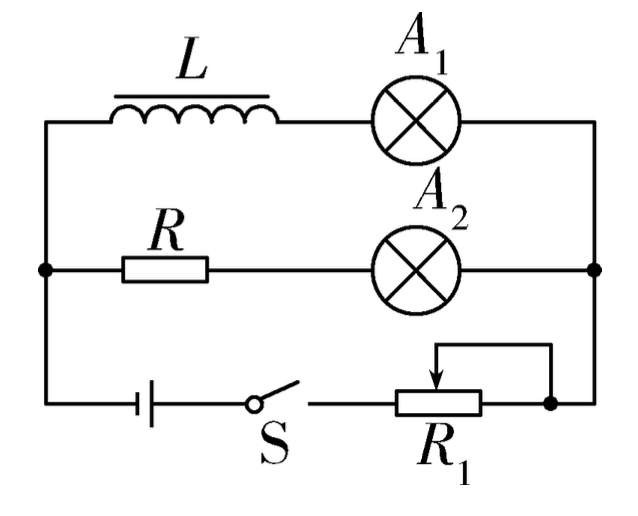
\includegraphics[width = \textwidth]{pictures/1.png}
        \caption*{Figure 1 $L$很大但无铁芯}
    \end{minipage}
    \hfill
    \begin{minipage}{0.43\textwidth}
        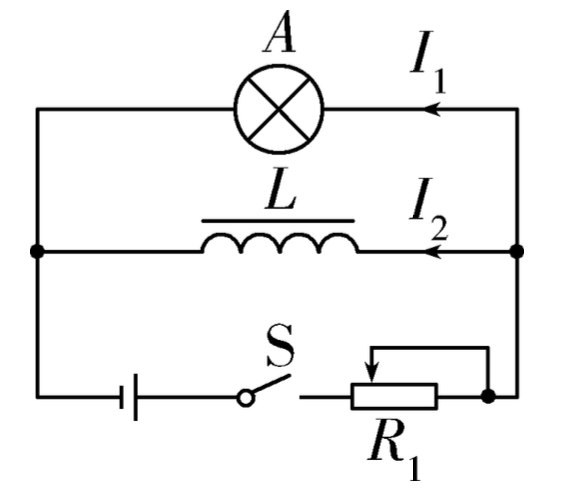
\includegraphics[width = \textwidth]{pictures/2.png}
        \caption*{Figure 2 $L$很大且有铁芯}
    \end{minipage}
\end{figure}

\begin{tabular*}{|c|c|c|}
            & 图1 & 图2   \\
    通电时   &     &       \\
    断电时   &     &       \\
\end{tabular*}




\end{document}